% =====================================================================
% THEIA — manuscript (ANONYMIZED main file)
% Target: Radiology: Artificial Intelligence, ORIGINAL RESEARCH
%   limits: 3000 words (Introduction–Discussion), 35 refs, 6 figures, 4 tables
%
% Radiology: AI uses DOUBLE-ANONYMIZED peer review. This file must contain
% NO author names, institutions, acknowledgments, or identifying URLs.
% The full title page (authors, affiliations, degrees, funding, conflicts,
% data sharing statement) lives in title_page.tex and is uploaded separately.
%
% Every number here is produced by ../scripts/reproduce.sh from ../results/.
% Nothing is transcribed by hand.
% =====================================================================
\documentclass[11pt]{article}

\usepackage[margin=1in]{geometry}
\usepackage{graphicx}
\usepackage{booktabs}
\usepackage{amsmath}
\usepackage{siunitx}
\usepackage[hidelinks]{hyperref}
\usepackage{caption}
\usepackage{float}
\usepackage[numbers,sort&compress]{natbib}
\usepackage{setspace}

\captionsetup{font=small,labelfont=bf}
\graphicspath{{../figures/}}
\sisetup{detect-weight=true}
\renewcommand{\arraystretch}{1.12}

\begin{document}

% ---------------------------------------------------------------------
% ABBREVIATED (ANONYMIZED) TITLE PAGE
% ---------------------------------------------------------------------
\begin{center}
{\LARGE\bfseries Weakly Supervised Localisation Generalises Where Genotype
Prediction Does Not: An Externally Validated Null for \textit{EGFR}
Radiogenomics from Lung CT\par}

\vspace{1em}
{\small Original Research $\cdot$ Manuscript type: Original Research \\
Word count (Introduction through Discussion): see title page \\
\textit{Author names and affiliations removed for anonymized review}}
\end{center}

\vspace{1em}
\hrule
\vspace{1em}

% ---------------------------------------------------------------------
\noindent\textbf{\large Summary Statement}

\medskip
\noindent\textbf{Weakly supervised tumour localisation transferred from a United
States surgical cohort to a Dutch radiotherapy cohort, whereas prediction of
epidermal growth factor receptor mutation status from the same lesion-anchored
computed tomographic images did not exceed a five-variable model built from
routinely recorded clinical data.}

\bigskip
\noindent\textbf{\large Key Points}

\begin{itemize}\itemsep3pt
  \item In 153 patients with a known \textit{EGFR} call, pooled out-of-fold AUC
    was $0.618 \pm 0.025$ versus $0.794$ for smoking status alone; adding the
    model to a five-variable clinical model changed AUC by $-0.029 \pm 0.015$,
    with every seed's confidence interval including zero.
  \item Supervised attention transferred to 420 external patients from a
    different country and scanner fleet, with an attention-mass lift of $+0.244$
    over a per-fold spatial shuffle and pointing accuracy of 0.609 versus 0.476
    for a centre prior and 0.005 for an untrained head.
  \item Across six defensible preprocessing choices the radiomics comparator
    moved 0.136 in AUC, exceeding the effect sizes this literature commonly
    reports as findings.
\end{itemize}

\medskip
\noindent\textbf{Abbreviations:} AUC = area under the receiver operating
characteristic curve, CI = confidence interval, CV = cross-validation,
IQR = interquartile range, NSCLC = non--small cell lung cancer,
ROI = region of interest, TKI = tyrosine kinase inhibitor.

\vspace{1em}
\hrule

% ---------------------------------------------------------------------
\section*{Abstract}

\noindent\textbf{Purpose.} To evaluate whether a grounded vision--language model
predicts \textit{EGFR} mutation status from lung CT beyond routinely available
clinical variables, and whether its supervised attention localises tumours on an
unseen cohort.

\noindent\textbf{Materials and Methods.} This retrospective secondary analysis
used the public NSCLC-Radiogenomics collection. Its CT dates are
de-identification offsets, so no accrual window is recoverable; the index
test--to--reference standard interval had a median of 38 days (IQR, 19.5--65.5).
Of 211 subjects, 153 had a known \textit{EGFR} call (mean age, 69 years $\pm$ 9
[SD]; 98 male, 55 female; 40 mutant [26.1\%]). A BiomedCLIP ViT-B/16 encoder with
a region-query grounding head supervised against tumour segmentations was trained
with nested five-fold cross-validation, three seeds. The primary endpoint was
external generalisation of localisation, assessed on 420 held-out
NSCLC-Radiomics patients against three controls: a per-fold spatial shuffle, a
centre prior, and an untrained head. A co-primary endpoint, incremental AUC over
a five-variable clinical model, was pre-declared as an expected null; the
analysis plan was fixed before external evaluation. $P < .05$ indicated
significance.

\noindent\textbf{Results.} Pooled out-of-fold \textit{EGFR} AUC was
$0.618 \pm 0.025$, versus 0.794 for smoking status alone. Adding the model to
clinical variables changed AUC by $-0.029 \pm 0.015$, every seed's CI including
zero; no fusion topology exceeded the clinical model. Calibration slope was 0.19,
and Brier score (0.236) exceeded the base-rate floor (0.193).
Localisation transferred: attention-mass lift was $+0.244$ over the shuffle in 11
of 15 external evaluations, with pointing accuracy 0.609 versus 0.476 (centre
prior) and 0.005 (untrained head).

\noindent\textbf{Conclusion.} Supervised localisation generalised across
institutions, whereas lesion-anchored \textit{EGFR} prediction did not exceed a
five-variable clinical model.

\vspace{1em}
\hrule
\vspace{1em}

% ---------------------------------------------------------------------
\section{Introduction}

\textit{EGFR} genotype directs tyrosine kinase inhibitor therapy in non--small
cell lung cancer (NSCLC). Tissue is often limited and molecular testing is not
universally available, so a non-invasive imaging surrogate would have real
clinical value. This has motivated a large radiogenomics literature.

That literature reports \textit{EGFR} prediction from CT at AUC 0.80--0.89
\citep{huang2025,shang2023,lai2026,wu2024,le2026}. The cohorts are typically
200--826 patients, usually single-centre, and external validation is uncommon.
Against this, the one large study with external validation --- 1{,}646 patients
and 11{,}473 segmented lesions with next-generation-sequencing labels --- reports
internal AUC 0.62--0.68 and external 0.55--0.63 \citep{rodriguez2026}. Notably,
its external cohort is NSCLC-Radiogenomics, the collection used here.

That discrepancy is this study's motivation. Reported performance in this field
is known to be sensitive to methodological choices that are invisible at internal
evaluation \citep{maleki2022,horvat2024}, which makes the separation of claims
more informative than another point estimate. We therefore do not propose a
better classifier. We separate two claims that are routinely bundled --- that
such a model \textit{localises} the lesion, and that it \textit{genotypes} it ---
and test each with the controls it requires, on a cohort where the second can be
measured against the clinical variables it would have to beat.

% ---------------------------------------------------------------------
\section{Materials and Methods}

\subsection{Ethics}

This study is a retrospective secondary analysis of publicly available, fully
de-identified imaging and clinical data distributed by The Cancer Imaging Archive
under open licences, and no protected health information was accessed at any
point.

\medskip
\noindent\fbox{\parbox{0.96\linewidth}{\small\textbf{[AUTHOR ACTION REQUIRED
BEFORE SUBMISSION]} Insert the institutional review board's written determination
here --- either formal approval, a waiver of informed consent, or a
not-human-subjects-research / exempt determination with its reference number and
date. Journal policy requires an explicit statement, and the authors' assessment
of the regulations is not a substitute for the board's. Also state
HIPAA-compliance status if any author's institution is in the United States.}}

\subsection{Study design and cohorts}

The analysis plan, including the primary endpoint and all controls, was fixed and
version-controlled before external evaluation; deviations from it are logged in
the public repository accompanying this work.

The internal cohort is NSCLC-Radiogenomics \citep{bakr2018}, a surgical series
distributed by The Cancer Imaging Archive. Participant flow is given in
Figure~\ref{fig:flow}: 211 subjects in the clinical sheet, 188 with an imaging
series, 158 successfully preprocessed, 153 with a known \textit{EGFR} call
(mean age, 69 years $\pm$ 9 [SD]; 98 male, 55 female), 133 adenocarcinoma, and 97
with both adenocarcinoma histology and a pixel-level segmentation. That last set
is the pre-specified primary analysis set. Cohort characteristics appear in
Table~\ref{tab:one}.

No accrual window is reported. The collection's CT dates span 1989--1996 and are
de-identification offsets rather than dates; publishing a range derived from them
would misdescribe the cohort. The interval from index test to reference standard,
which survives the offset because it is a difference, has a median of 38 days
(IQR, 19.5--65.5).

The external cohort is NSCLC-Radiomics \citep{aerts2014}, 420 preprocessed
patients from a Dutch centre --- a different country, scanner fleet, and clinical
population (radiotherapy planning rather than surgical). The two cohorts share no
patients, and no evaluated checkpoint was warm-started from the external
collection; both facts are asserted in the accompanying automated test suite
rather than claimed in prose.

\subsection{Reference standard}

\textit{EGFR} status was determined by sequencing and is distributed with the
collection \citep{bakr2018}. The grounding reference standard is the expert
tumour segmentation distributed with each collection. Only one contour per lesion
exists, so inter-rater agreement cannot be computed; a mask perturbation sweep is
reported instead and is explicitly not a substitute (Discussion).

\subsection{Model}

A BiomedCLIP ViT-B/16 encoder (last two blocks unfrozen) produces patch tokens
per section, aggregated across 16 sections by a masked mean. A grounding head
applies eight learned region queries by cross-attention, and the resulting
attention maps are supervised against the tumour region of interest (ROI)
projected onto the patch grid. The classifier pools from the grounded region
embeddings, so prediction and localisation share a representation.

Inputs are axial crops of $(\text{bbox}_{\text{mm}} + 24)\times 2.5$ around the
lesion with 30\% positional jitter, windowed at centre $-600$~HU / width
1500~HU and resized to $224\times224$.

\subsection{Endpoints and controls}

\textbf{H\textsubscript{1} (primary).} External attention-mass lift over a
per-fold spatial shuffle is greater than zero. Three controls are mandatory in
every reported table:

\begin{itemize}\itemsep2pt
  \item \textbf{Spatial shuffle} --- the same attention values permuted across
    cells, isolating \textit{where} mass fell from \textit{how peaked} the map is.
  \item \textbf{Centre prior} --- external ROI centroids sit at $(0.50, 0.51)$ of
    the frame ($\text{SD} \approx 0.08$) covering 4.9\% of area, so ``look at the
    middle'' is a strong baseline. Pointing accuracy and area-matched
    intersection over union are invariant to the prior's width, so that margin
    cannot be tuned.
  \item \textbf{Weight randomisation} --- an untrained head of identical
    architecture, ruling out architectural inductive bias.
\end{itemize}

\textbf{H\textsubscript{2} (co-primary, pre-declared null).}
$\Delta\text{AUC} = \text{AUC}(\text{clinical}+\text{model}) -
\text{AUC}(\text{clinical})$.

\subsection{Statistical analysis}

Evaluation used nested five-fold cross-validation (CV) stratified on
\textit{EGFR}, three seeds, with within-fold rank normalisation before pooling.
The headline is the across-seed mean $\pm$ SD; a pooled confidence interval (CI)
absorbs no rerun variance and is never quoted alone. \textbf{No operating point
is defined}: the index test is continuous and the calibration reported in
Section~\ref{sec:calib} does not support a threshold, so sensitivity and
specificity are not reported.

Comparisons used a paired bootstrap over patients (2000 resamples), with Holm
correction across the ten arms of the pooling sweep. Precision was computed by
the Hanley--McNeil closed form \citep{hanley1982}, validated against a bootstrap;
minimum sample size follows Riley et al.\ \citep{riley2020}, applied only where
its inputs are defined. Reporting follows the Checklist for Artificial
Intelligence in Medical Imaging \citep{claim2020}; the completed checklist is
submitted with this manuscript.

Two-sided $P < .05$ was considered to indicate a significant difference.
Analyses were performed in Python 3.13.9 (Python Software Foundation) with NumPy
2.1.3, SciPy 1.15.3, scikit-learn 1.6.1, pandas 2.2.3 and statsmodels 0.14.4 (all
open-source, respective maintainers), and PyTorch 2.10.0 (Meta Platforms).

% ---------------------------------------------------------------------
\section{Results}

\subsection{The model does not exceed the clinical variables}

Table~\ref{tab:arms} gives every arm on identical patients and folds.
Pooled out-of-fold \textit{EGFR} AUC was $0.618 \pm 0.025$ across three seeds.
Smoking status alone reached 0.794; the five-variable clinical model 0.764.

The co-primary endpoint was $\Delta\text{AUC} = -0.029 \pm 0.015$, with every
seed's CI including zero. No fusion topology exceeded the clinical model: soft
voting reached 0.748, cross-fitted stacking 0.735, hard voting 0.690. Adding
radiomics significantly \textit{harmed} the combination ($-0.130$, $P = .02$). A
logistic regression on frozen encoder features scored $0.617 \pm 0.052$ ---
indistinguishable from the full network to three decimals.

Results are shown per arm in Figure~\ref{fig:roc} and with paired deltas in
Figure~\ref{fig:forest}. \textit{KRAS} was at chance ($0.489 \pm 0.005$); Gevaert
et al.\ likewise report no significant \textit{KRAS} model on this cohort
\citep{gevaert2017}.

\subsection{The predictions are also uncalibrated}\label{sec:calib}

Calibration slope averaged 0.19 against a perfect 1.0, indicating predictions
roughly five times too extreme. At a base rate of 26.1\%, a model predicting the
prevalence for every patient achieves a Brier score of 0.193; the model scored
0.236. \textbf{The probabilities are therefore worse than a constant}, with
resolution --- the component only a better model can improve --- between 0.009
and 0.017. This is why no operating point is pre-specified, and why any future
externally validated artifact must carry explicit recalibration.

\subsection{On the subset that should carry it, performance is weaker}

Every \textit{EGFR}-mutant patient in this collection is an adenocarcinoma; the
17 squamous and 3 NSCLC-not-otherwise-specified patients are wild-type without
exception. Including them makes 13\% of the cohort classifiable from histology
alone with no imaging. On the pre-specified primary analysis set --- segmented
adenocarcinoma, $n = 97$, 23 positives --- AUC falls to 0.563. The same pattern
appears in the literature: Yamazaki et al.\ report 0.774 across histologies but
0.687 restricted to adenocarcinoma \citep{yamazaki2022}.

\subsection{Localisation generalises to an unseen cohort}

On 420 held-out NSCLC-Radiomics patients (Figure~\ref{fig:external}), attention
mass inside the tumour was 0.292 against 0.048 for the spatial shuffle --- a lift
of $+0.244$, beating the shuffle in 11 of 15 evaluations. Pointing accuracy
reached 0.609 against 0.476 for the centre prior and 0.005 for a randomly
initialised head, which returned a lift of exactly $+0.000$ at a peak-to-mean
ratio of 1.01.

\textbf{The margin over the pre-specified fold-rate threshold is one fold}:
11 of 15 (73.3\%) against a required 71.4\%. Because that margin invites the
reading that the endpoint is knife-edge, Table~\ref{tab:external} reports every
evaluation individually. The distribution is bimodal rather than marginal. The
weakest success has a lift of $+0.258$ and pointing accuracy of 0.757; the
strongest failure has a lift of $-0.005$ and pointing accuracy of exactly 0.000.
No evaluation falls between 0.000 and 0.757 on pointing accuracy. Folds either
localise decisively or not at all, so the endpoint is insensitive to where the
threshold is placed within a wide interval, while remaining sensitive to how many
folds land on each side.

The failures are also concentrated rather than scattered: one training run
localised in 2 of 5 folds while the others reached 5 of 5 and 4 of 5, and that
same run localises in 2 of 5 internally while carrying the \textit{highest}
classification AUC of the three. Localisation is therefore a property of most
training runs rather than of the method.

Representative attention maps appear in Figure~\ref{fig:overlays}. These are the
first six segmented patients of a held-out fold in index order, not selected on
score.

\subsection{The peritumoral region carries the signal, but not significantly}

Because the classifier pools from the grounded region --- the lesion itself ---
we asked whether the \textit{EGFR} signal is located where the grounding loss
supervises attention. Over ten seeds on frozen encoder features, through
identical nested folds, mean-pooling the peritumoral ring scored 0.695 against
0.632 for the whole crop and 0.629 for the tumour interior. A size- and
shape-matched ring at a \textit{random} location scored 0.575, so the gain is
location-specific rather than an artefact of pooling a thin annulus. Adding a
peritumoral branch to the classifier moved the trained model from 0.618 to
$0.675 \pm 0.017$, improving in 3 of 3 seeds.

\textbf{This does not survive correction, and we report it as suggestive rather
than established.} The sweep scores ten arms on the same folds; under a paired
bootstrap over patients with Holm correction, the best arm has $P_{\text{raw}} =
.03$ and $P_{\text{Holm}} = .28$. End-to-end the branch is worth $+0.058$ (95\%
CI: $-0.008$, $+0.128$; $P = .09$). The direction is consistent across frozen and
trained settings and the location controls behave; the significance is absent.

It is also a replication rather than a discovery: peritumoral radiomics for
\textit{EGFR} has been reported at least six times since 2022, with optimal ring
widths of 1, 2, 3, 4, 6 and 15~mm
\citep{yamazaki2022,shang2023,wu2024,le2026,lai2026,huang2025}. What is new here
is the tension it exposes --- the grounding objective supervises attention
\textit{onto} the lesion, and the classification signal appears to sit just
outside it.

\subsection{Analytic choice is worth more than the effect}

On identical features and estimator, the radiomics arm moved \textbf{0.136 in
AUC} across six defensible preprocessing choices, and \textbf{0.066} between a
flat and a nested CV protocol. Both exceed the effect sizes this literature
reports as findings, and both are of the kind that internal evaluation cannot
detect \citep{maleki2022}.

\subsection{More patients would not settle it}

Riley's criterion requires 414 patients for the five-variable clinical model
alone and 42{,}362 for the 512-feature frozen probe; this cohort has 153. Neither
arm is identifiable at this sample size, which is why ``the probe matches the
model'' cannot be read as evidence that the architecture is redundant.

Precision, not power, binds any external test. At the observed prevalence a 95\%
CI half-width of $\pm0.05$ requires $n = 661$. The entire open world of
\textit{EGFR}-labelled CT holds approximately 327 cases with 64 positives, giving
$\pm0.154$ --- an interval spanning chance and the published 0.80s
simultaneously.

% ---------------------------------------------------------------------
\section{Discussion}

Two claims usually bundled together separate cleanly here, and separate
differently. Supervised localisation transferred to a cohort from another
country, scanner fleet and treatment setting. Genotype prediction did not clear a
five-variable clinical model on the cohort it was trained on
($\Delta\text{AUC} = -0.029 \pm 0.015$), was not rescued by any fusion topology,
and was worse than a constant on the probability scale (Brier 0.236 vs a
base-rate floor of 0.193).

\textbf{What the localisation endpoint does and does not establish.} Attention
mass, pointing accuracy and area-matched intersection over union are not measures
of diagnostic accuracy, and no clinical claim follows from them directly. They
answer a narrower question that we think has been assumed rather than tested:
whether the explanation a model offers for its prediction is anchored to the
lesion at all, on data from an institution it has never seen. That question
matters precisely because the accompanying prediction fails. A saliency map that
tracks the tumour on an unseen cohort while the classifier built on it performs
at 0.618 is direct evidence that plausible localisation is not evidence of
predictive validity --- a dissociation that cannot be observed in a study where
both are reported as successes. We therefore present H\textsubscript{1} as a
methodological result about interpretability claims, not as a clinical endpoint,
and we do not propose the localiser for clinical use.

\textbf{Convergence with the largest external study.} Rodríguez Sánchez et al.\
\citep{rodriguez2026} is the strongest argument that this is a property of the
problem rather than of our sample. Their 1{,}646 patients and 11{,}473 lesions,
with next-generation-sequencing labels and biopsy-anchored training, reproduce
the interval we obtain from 153 patients; their external cohort is the collection
we use internally. Ten times the patients did not move the ceiling. Read together
with the measured precision bound above --- $\pm0.154$ on the largest test set
the open literature can currently assemble --- the implication is that the field
cannot resolve this question with public data, and that the reported 0.80s are
more plausibly explained by analytic variation than by a signal the larger
studies missed.

\textbf{Comparison with prior reports.} Our peritumoral finding replicates six
prior reports in direction while failing to reach significance after correction
for the ten arms actually examined. We consider that a more likely description of
this literature than the alternative, given that the same six reports place the
optimal ring width anywhere from 1 to 15~mm. Similarly, our histology result
reproduces Yamazaki et al.\ \citep{yamazaki2022}: performance falls when the
squamous patients, who are wild-type without exception, are removed. Any study
reporting \textit{EGFR} AUC across mixed histologies is partly reporting a
histology classifier.

\textbf{Limitations.} The internal cohort is single-institution and historical,
and no accrual window is recoverable from it. The classification arm has no
external validation; that is justified by the measured precision bound above
rather than by circumstance, and is reported as a finding rather than deferred.
Inter-rater variability of the segmentations is not measured, because the source
collections distribute one contour per lesion; a mask perturbation sweep
(dilation, erosion, translation) is reported instead and is explicitly not a
substitute for a second reader. Acquisition parameters --- section thickness,
convolution kernel, vendor --- are incompletely recoverable. One of three training
runs largely fails to localise, and we report the endpoint on all three rather
than on the two that succeed. Finally, H\textsubscript{1} is confirmatory of a
prior observation on an independent patient set rather than a blind prospective
test: the external cohort was on disk, and the metric's behaviour on it partly
known, when the threshold was set. The registered plan states this precisely, and
we state it here rather than let a reader infer a stronger design than was run.

\textbf{Conclusion.} On this cohort, weakly supervised localisation generalised
across institutions while \textit{EGFR} prediction from lesion-anchored CT did
not exceed routinely available clinical variables. Reports of AUC 0.80--0.89
should be read against the analytic-choice sensitivity and precision bounds
measured here.

% ---------------------------------------------------------------------
\section*{Data and code availability}

All code, the pre-specified analysis plan with its deviation log, the completed
CLAIM checklist, and every archived run result --- including negative results ---
are available at an anonymized repository for review
(\texttt{[ANONYMIZED REPOSITORY LINK --- see cover letter]}); the permanent
public URL and archival DOI will be provided on acceptance. Every number in this
manuscript is regenerated by a single script from archived out-of-fold
predictions, requiring no imaging data and no GPU.

Imaging is redistributed by The Cancer Imaging Archive under its own terms and is
not included in the repository. NSCLC-Radiogenomics is CC BY 3.0;
NSCLC-Radiomics is CC BY-NC 3.0. Figure~\ref{fig:overlays} shows
NSCLC-Radiogenomics images only, consistent with that licence.

% ---------------------------------------------------------------------
\clearpage
\section*{Figures}

\begin{figure}[H]\centering
  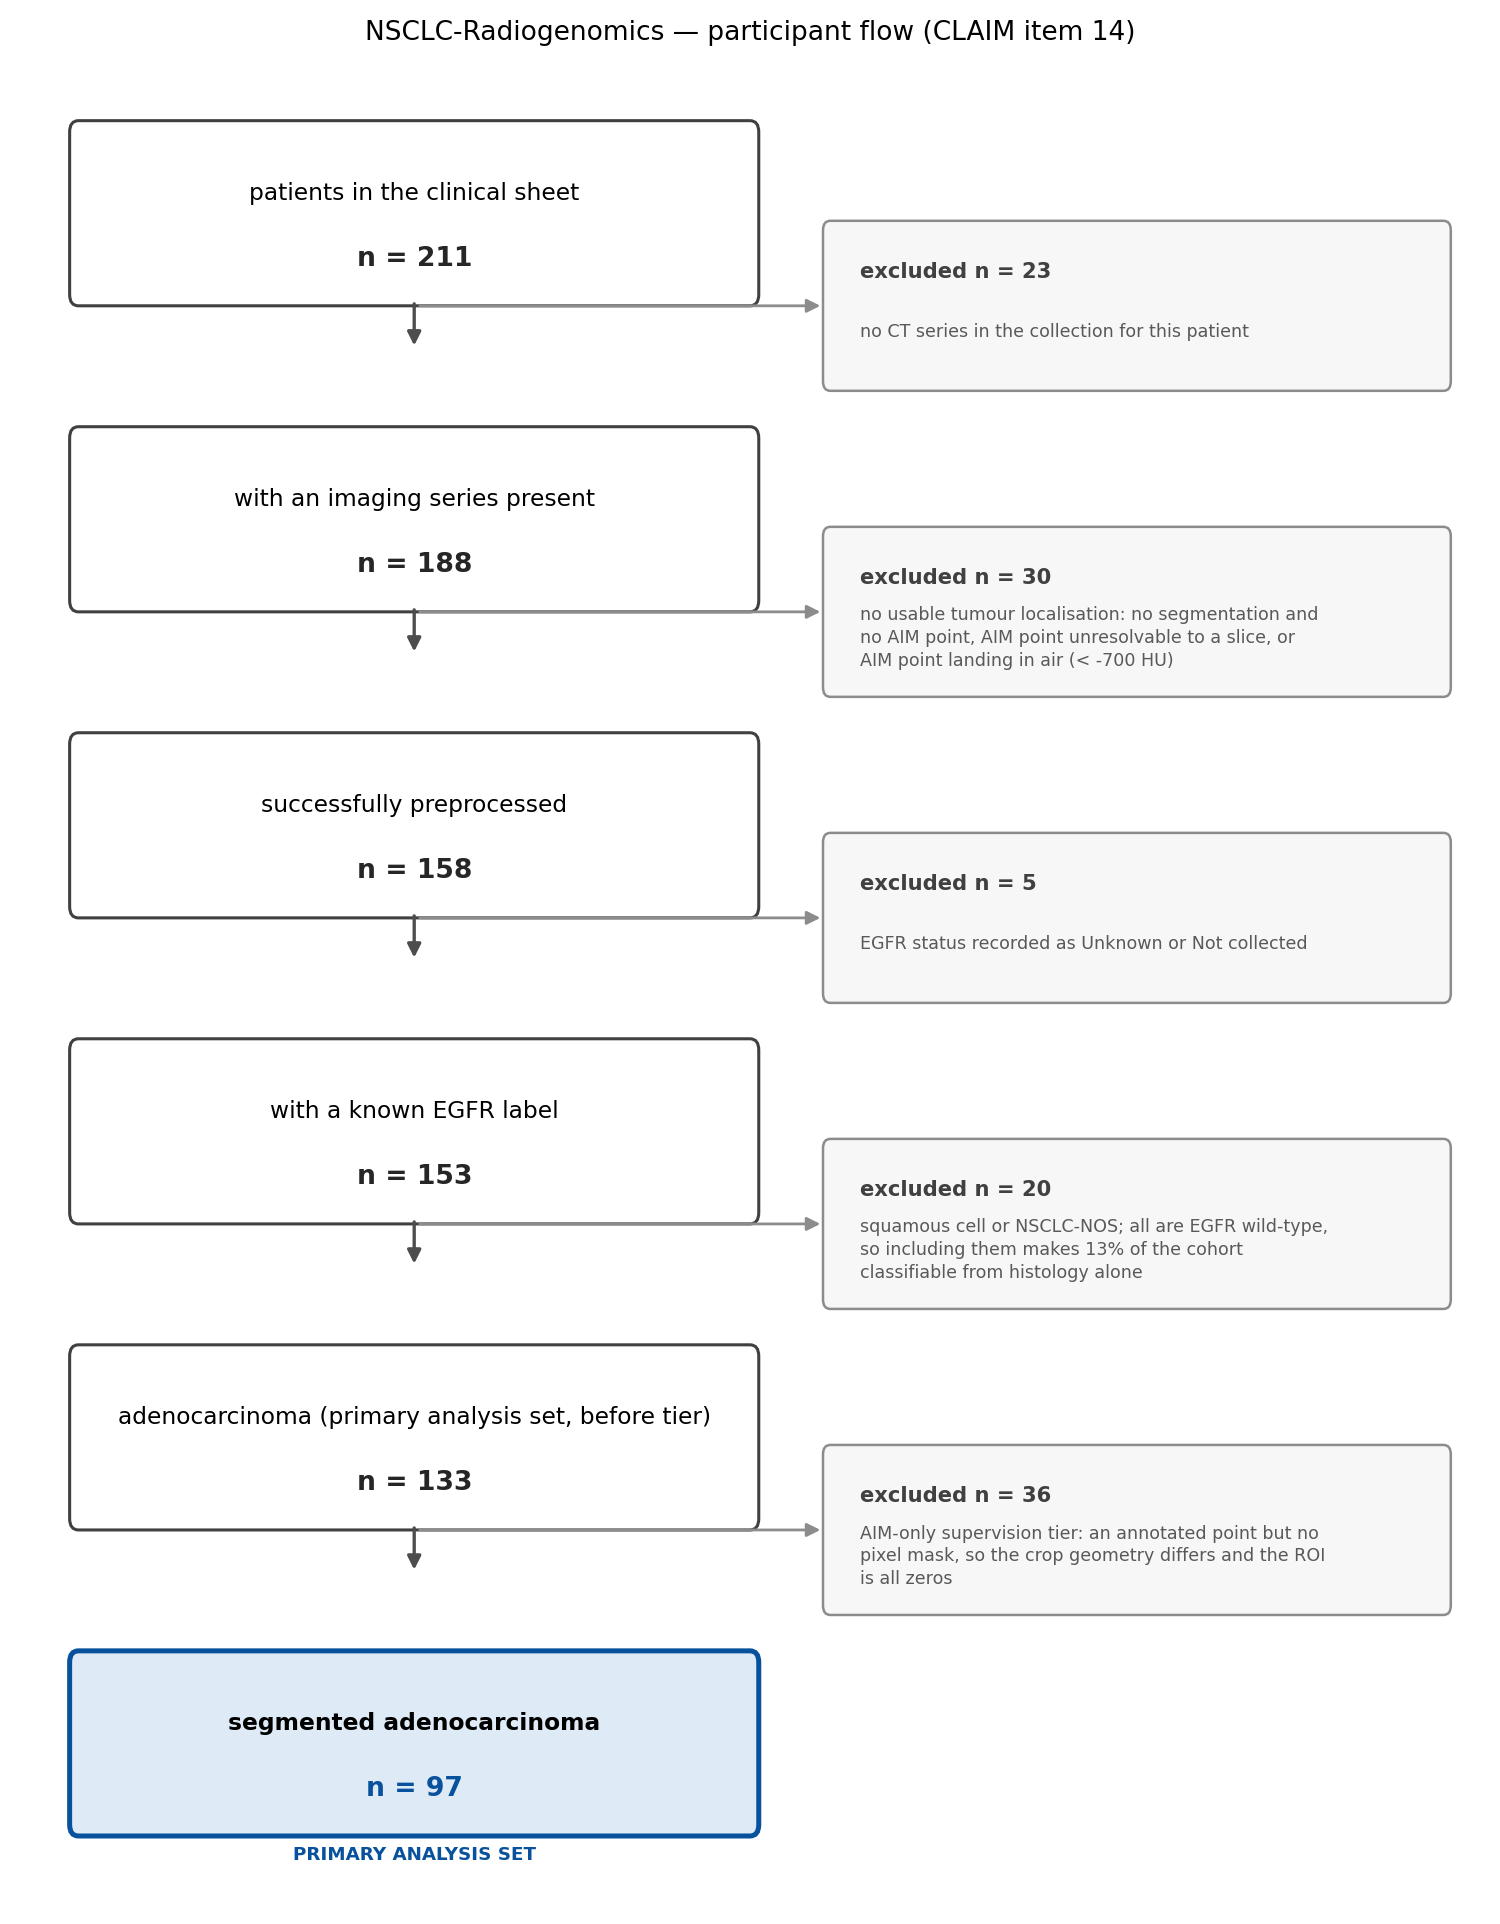
\includegraphics[width=0.72\textwidth]{fig1_flow.png}
  \caption{\textbf{Participant flow.} Counts and exclusion reasons are generated
  from the pipeline rather than transcribed, and reconcile exactly
  ($211 - 114 = 97$). The pre-specified primary analysis set is segmented
  adenocarcinoma.}
  \label{fig:flow}
\end{figure}

\begin{figure}[H]\centering
  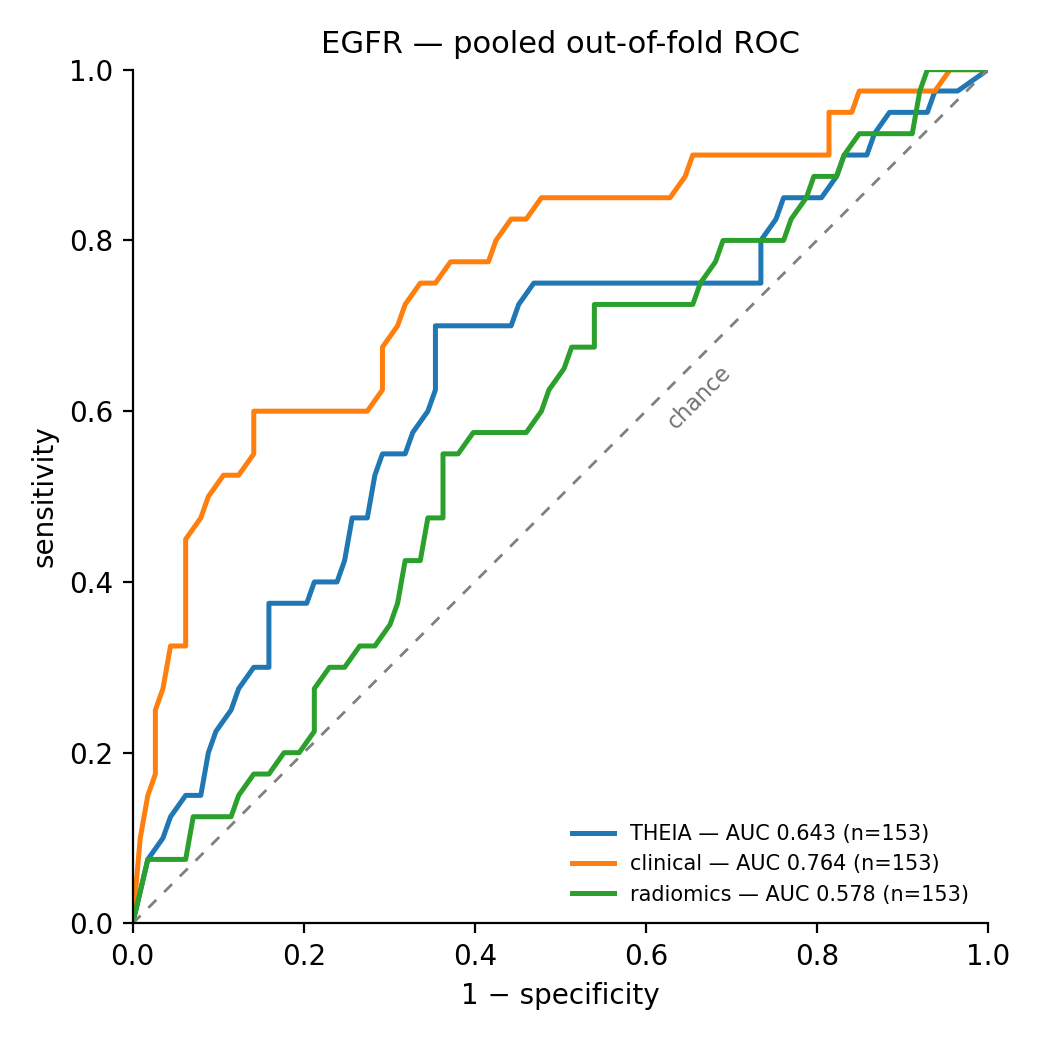
\includegraphics[width=0.62\textwidth]{fig1_roc.png}
  \caption{\textbf{Pooled out-of-fold receiver operating characteristic curves by
  arm}, on identical patients and folds. The chance line is drawn and labelled;
  each arm's $n$ is printed, because arms do not all cover the same patients.}
  \label{fig:roc}
\end{figure}

\begin{figure}[H]\centering
  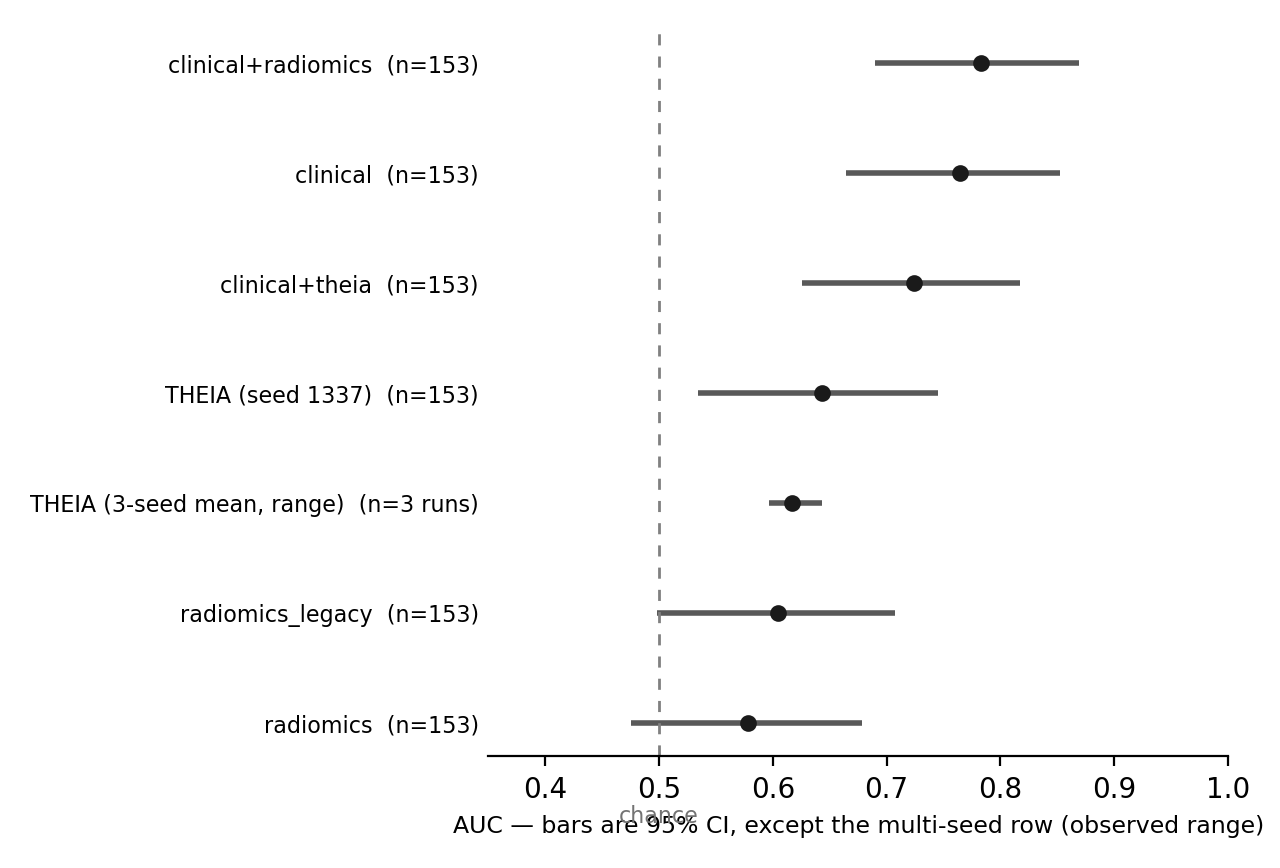
\includegraphics[width=0.86\textwidth]{fig2_forest.png}
  \caption{\textbf{Every arm with its confidence interval.} Overlapping intervals
  can still differ significantly when paired, which is why the paired deltas are
  reported alongside.}
  \label{fig:forest}
\end{figure}

\begin{figure}[H]\centering
  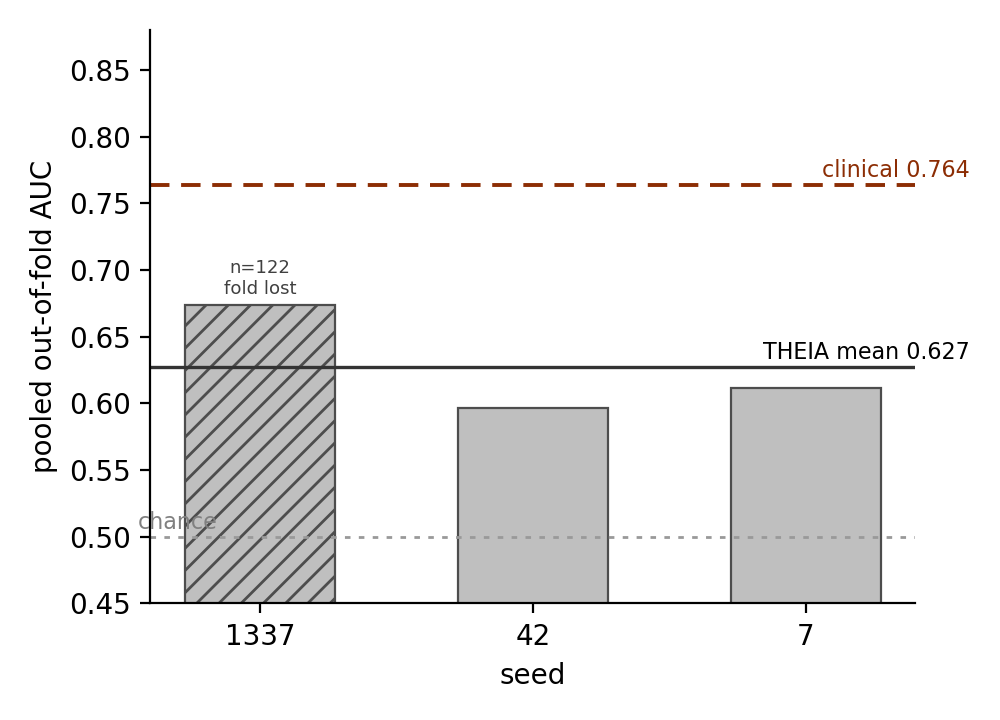
\includegraphics[width=0.62\textwidth]{fig3_seeds.png}
  \caption{\textbf{Per-seed AUC against the clinical baseline.} The rerun spread
  is shown next to the effect being claimed; the gap to a five-variable clinical
  model exceeds it.}
  \label{fig:seeds}
\end{figure}

\begin{figure}[H]\centering
  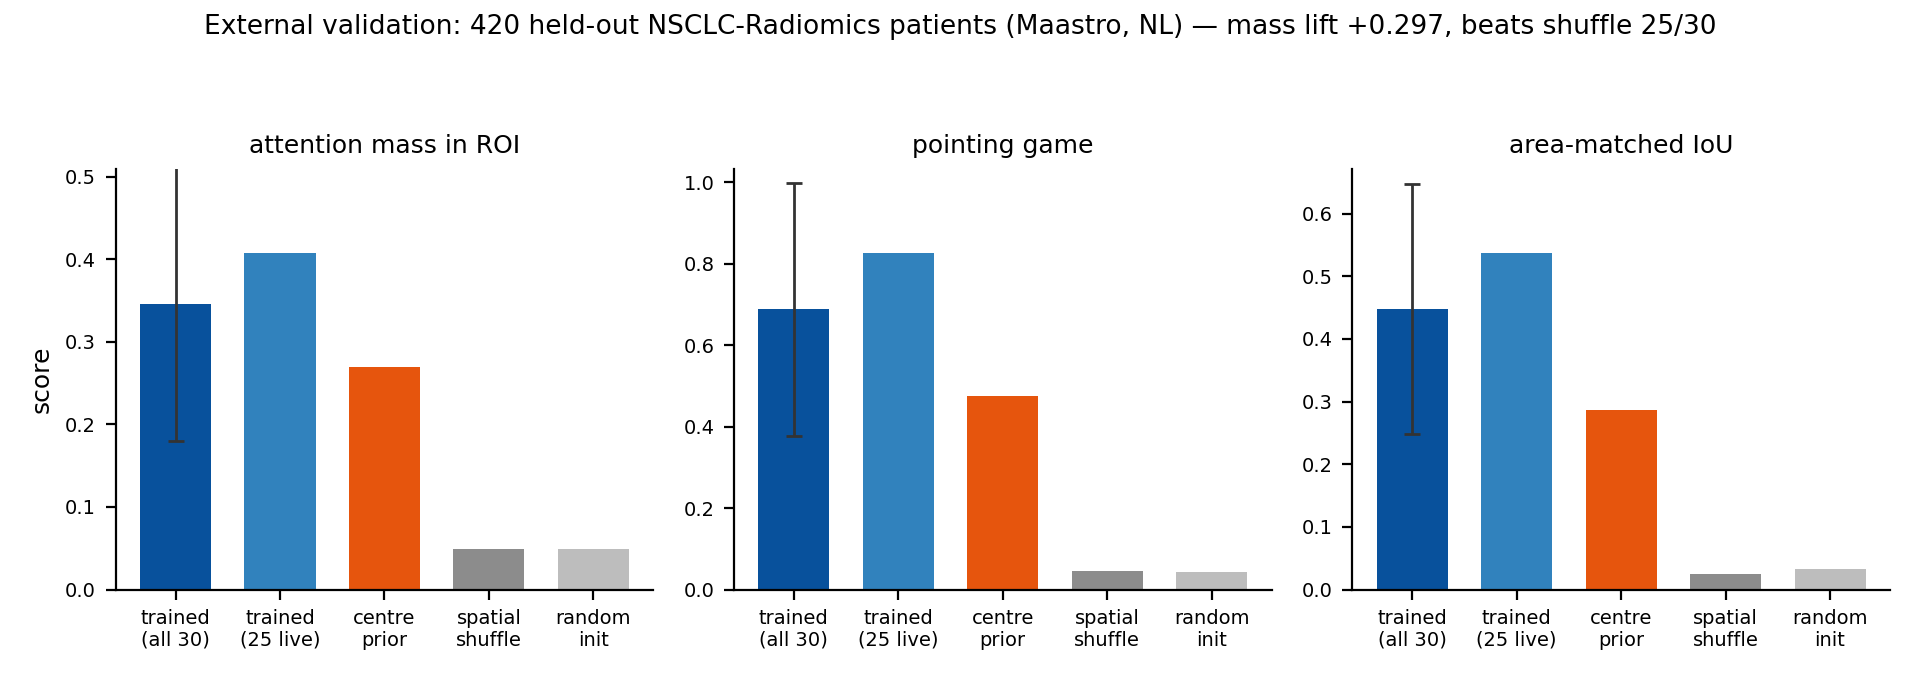
\includegraphics[width=\textwidth]{fig6_external_grounding.png}
  \caption{\textbf{Primary endpoint: localisation on 420 held-out
  NSCLC-Radiomics patients}, with all three controls in every panel. The centre
  prior is strong on attention mass by construction and weak on pointing accuracy
  and area-matched intersection over union, which are invariant to its width ---
  so the trained model's margin is read from the right-hand panels, not the
  left.}
  \label{fig:external}
\end{figure}

\begin{figure}[H]\centering
  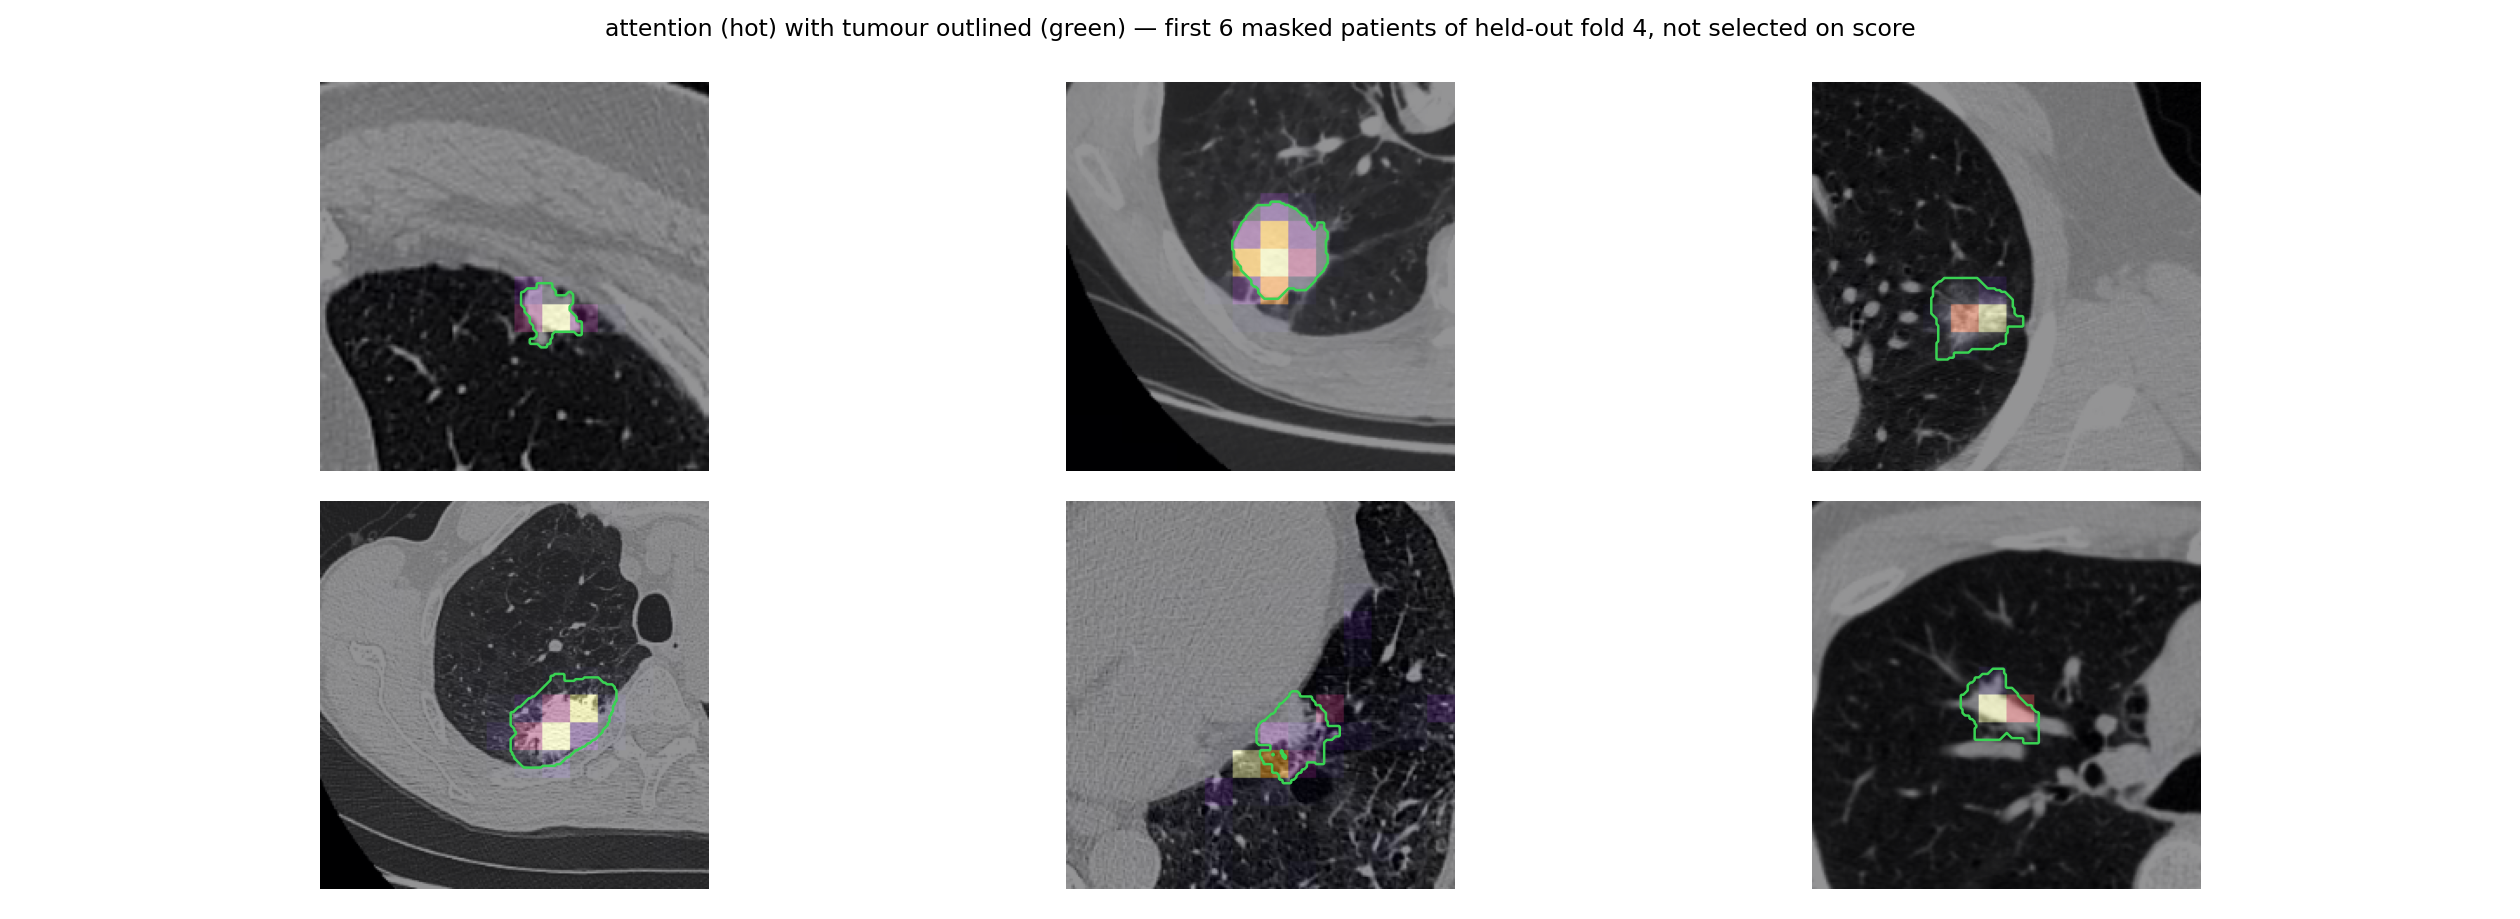
\includegraphics[width=\textwidth]{fig5_overlays.png}
  \caption{\textbf{Attention maps with the tumour contour drawn from the
  reference segmentation.} The first six segmented patients of a held-out fold in
  index order, \textit{not} selected on score. Images from NSCLC-Radiogenomics
  (CC BY 3.0) \citep{bakr2018}.}
  \label{fig:overlays}
\end{figure}

% ---------------------------------------------------------------------
\clearpage
\section*{Tables}

\begin{table}[H]\centering\small
\caption{\textbf{Cohort characteristics by \textit{EGFR} status}, restricted to
the 153 patients with a known call. Never-smokers are 50\% of mutants against
12\% of wild-type; this is the textbook epidemiology and is most of what the
clinical model knows.}
\label{tab:one}
\begin{tabular}{lccc}
\toprule
\textbf{Characteristic} & \textbf{\textit{EGFR} mutant} & \textbf{Wild-type} & \textbf{All} \\
\midrule
$n$                          & 40         & 113        & 153 \\
Age (y), mean $\pm$ SD       & --- & --- & 69 $\pm$ 9 \\
Age (y), median [IQR]        & 68 [63--76] & 69 [64--75] & 69 [64--76] \\
Pack-years, median [IQR]     & 15 [9--34]  & 42 [26--56] & 40 [20--50] \\
\midrule
Female                       & 22 (55\%)  & 33 (29\%)  & 55 (36\%) \\
Male                         & 18 (45\%)  & 80 (71\%)  & 98 (64\%) \\
\midrule
Never-smoker                 & 20 (50\%)  & 13 (12\%)  & 33 (22\%) \\
Former smoker                & 18 (45\%)  & 78 (69\%)  & 96 (63\%) \\
Current smoker               & 2 (5\%)    & 22 (19\%)  & 24 (16\%) \\
\midrule
Asian                        & 9 (22\%)   & 6 (5\%)    & 15 (10\%) \\
Caucasian                    & 13 (32\%)  & 77 (68\%)  & 90 (59\%) \\
Other / not recorded         & 18 (45\%)  & 30 (27\%)  & 48 (31\%) \\
\midrule
Adenocarcinoma               & 40 (100\%) & 93 (82\%)  & 133 (87\%) \\
Squamous cell carcinoma      & 0 (0\%)    & 17 (15\%)  & 17 (11\%) \\
NSCLC not otherwise specified & 0 (0\%)   & 3 (3\%)    & 3 (2\%) \\
\bottomrule
\end{tabular}

\smallskip
\parbox{0.92\textwidth}{\footnotesize Note.---IQR = interquartile range,
NSCLC = non--small cell lung cancer. Percentages are column percentages within
each \textit{EGFR} group. Age is summarised by both mean $\pm$ SD and median
[IQR] because the distribution is mildly left-skewed; per-group means are omitted
to avoid implying a comparison that was not tested.}
\end{table}

\begin{table}[H]\centering\small
\caption{\textbf{All arms and fusion topologies}, on identical patients and folds.
No combination of the imaging model with clinical variables exceeds the clinical
model alone, and adding radiomics significantly harms it.}
\label{tab:arms}
\begin{tabular}{lccc}
\toprule
\textbf{Arm} & \textbf{\textit{EGFR} AUC} & \textbf{$\Delta$ vs clinical} & \textbf{$P$ value} \\
\midrule
\multicolumn{4}{l}{\textit{Single arms}}\\
Smoking status alone            & \textbf{0.794} & $+0.030$ & --- \\
Clinical (5 variables)          & 0.764 & --- & --- \\
THEIA, 3 seeds                  & $0.618 \pm 0.025$ & $-0.108$ & --- \\
\quad + peritumoral branch      & $0.675 \pm 0.017$ & $-0.089$ & --- \\
Frozen-feature logistic probe   & $0.617 \pm 0.052$ & $-0.147$ & --- \\
Radiomics                       & 0.578 & $-0.186$ & --- \\
\midrule
\multicolumn{4}{l}{\textit{Fusion topologies}}\\
Soft voting (model + clinical)  & 0.748 & $-0.016$ & .59 \\
Stacking (cross-fitted)         & 0.735 & $-0.029$ & .11 \\
Soft voting (equal weights)     & 0.712 & $-0.052$ & .15 \\
Soft voting (clinical + radiomics) & 0.703 & $-0.061$ & \textbf{.02} \\
Hard voting                     & 0.690 & $-0.074$ & .07 \\
Soft voting (model + radiomics) & 0.634 & $-0.130$ & \textbf{.02} \\
\midrule
\multicolumn{4}{l}{\textit{Co-primary endpoint}}\\
$\Delta$AUC (clinical + model) $-$ clinical & \multicolumn{3}{c}{$\mathbf{-0.029 \pm 0.015}$, every seed's CI includes zero} \\
\bottomrule
\end{tabular}

\smallskip
\parbox{0.92\textwidth}{\footnotesize Note.---AUC = area under the receiver
operating characteristic curve, CI = confidence interval. $\Delta$ is against the
clinical model. $P$ values are from a paired bootstrap over patients (2000
resamples); two-sided $P < .05$ indicated significance. Values with $\pm$ are
across-seed mean $\pm$ SD over three seeds.}
\end{table}

\begin{table}[H]\centering\small
\caption{\textbf{Primary endpoint, every external evaluation individually}, on
the same 420 held-out NSCLC-Radiomics patients. The margin over the pre-specified
fold-rate threshold is one evaluation, so each is shown rather than summarised.
Success and failure are separated by a wide gap on every metric: no evaluation
falls between 0.000 and 0.757 on pointing accuracy.}
\label{tab:external}
\begin{tabular}{llccccc}
\toprule
\textbf{Run} & \textbf{Fold} & \textbf{Mass} & \textbf{Shuffle} & \textbf{Lift} & \textbf{Pointing} & \textbf{IoU} \\
\midrule
A & 0 & 0.375 & 0.048 & $+0.327$ & 0.862 & 0.563 \\
A & 1 & 0.038 & 0.045 & $-0.007$ & 0.000 & 0.001 \\
A & 2 & 0.394 & 0.048 & $+0.346$ & 0.855 & 0.543 \\
A & 3 & 0.038 & 0.045 & $-0.007$ & 0.000 & 0.000 \\
A & 4 & 0.043 & 0.048 & $-0.005$ & 0.000 & 0.000 \\
\midrule
B & 0 & 0.327 & 0.049 & $+0.278$ & 0.833 & 0.538 \\
B & 1 & 0.316 & 0.048 & $+0.268$ & 0.790 & 0.502 \\
B & 2 & 0.401 & 0.050 & $+0.351$ & 0.893 & 0.570 \\
B & 3 & 0.411 & 0.051 & $+0.360$ & 0.831 & 0.562 \\
B & 4 & 0.550 & 0.049 & $+0.501$ & 0.802 & 0.525 \\
\midrule
C & 0 & 0.345 & 0.049 & $+0.296$ & 0.810 & 0.524 \\
C & 1 & 0.040 & 0.044 & $-0.005$ & 0.000 & 0.016 \\
C & 2 & 0.306 & 0.049 & $+0.258$ & 0.757 & 0.469 \\
C & 3 & 0.409 & 0.051 & $+0.359$ & 0.829 & 0.550 \\
C & 4 & 0.384 & 0.048 & $+0.336$ & 0.874 & 0.553 \\
\midrule
\multicolumn{2}{l}{\textbf{Trained, mean}} & 0.292 & 0.048 & $\mathbf{+0.244}$ & \textbf{0.609} & 0.394 \\
\multicolumn{2}{l}{\textit{Control:} centre prior} & 0.270 & 0.056 & $+0.214$ & 0.476 & 0.287 \\
\multicolumn{2}{l}{\textit{Control:} untrained head} & 0.049 & 0.049 & $-0.000$ & 0.005 & 0.008 \\
\bottomrule
\end{tabular}

\smallskip
\parbox{0.92\textwidth}{\footnotesize Note.---IoU = area-matched intersection
over union. Runs A, B and C are three independently seeded training runs of five
cross-validation folds each. Mass is the fraction of attention falling inside the
reference tumour contour; Shuffle is the same values permuted across cells; Lift
is their difference. Eleven of 15 evaluations exceed their shuffle, meeting the
pre-specified threshold of 71.4\% by one evaluation. All 11 successes exceed the
centre prior on pointing accuracy.}
\end{table}

% ---------------------------------------------------------------------
\clearpage
\bibliographystyle{unsrtnat}
\begin{thebibliography}{20}

\bibitem[Bakr et al.(2018)]{bakr2018}
Bakr S, Gevaert O, Echegaray S, et al.
A radiogenomic dataset of non-small cell lung cancer.
\textit{Sci Data} 2018;5:180202. doi:10.1038/sdata.2018.202

\bibitem[Gevaert et al.(2017)]{gevaert2017}
Gevaert O, Echegaray S, Khuong A, et al.
Predictive radiogenomics modeling of EGFR mutation status in lung cancer.
\textit{Sci Rep} 2017;7:41674. doi:10.1038/srep41674

\bibitem[Aerts et al.(2014)]{aerts2014}
Aerts HJWL, Wee L, Rios Velazquez E, et al.
Data From NSCLC-Radiomics (version 4). The Cancer Imaging Archive, 2014.
doi:10.7937/K9/TCIA.2015.PF0M9REI

\bibitem[Rodríguez Sánchez et al.(2026)]{rodriguez2026}
Rodríguez Sánchez DI, Middelkoop J, Vanneste T, et al.
Quality over quantity: biopsy-anchored CT radiogenomics models outperform
all-lesion training in a multi-tumour cohort despite a smaller sample size.
\textit{Eur Radiol} 2026. doi:10.1007/s00330-026-12601-9

\bibitem[Huang et al.(2025)]{huang2025}
Huang L, Xu L, Wang X, et al.
Prediction of EGFR mutations in lung adenocarcinoma via CT images.
\textit{Acad Radiol} 2025;32(8):4880--4892. doi:10.1016/j.acra.2025.04.029

\bibitem[Shang et al.(2023)]{shang2023}
Shang Y, Chen W, Li G, et al.
Computed tomography-derived intratumoral and peritumoral radiomics in predicting
EGFR mutation in lung adenocarcinoma.
\textit{Radiol Med} 2023;128(12):1483--1496. doi:10.1007/s11547-023-01722-6

\bibitem[Yamazaki et al.(2022)]{yamazaki2022}
Yamazaki M, Yagi T, Tominaga M, et al.
Role of intratumoral and peritumoral CT radiomics for the prediction of EGFR gene
mutation in primary lung cancer.
\textit{Br J Radiol} 2022;95(1140):20220374. doi:10.1259/bjr.20220374

\bibitem[Wu et al.(2024)]{wu2024}
Wu J, Meng H, Zhou L, et al.
Habitat radiomics and deep learning fusion nomogram to predict EGFR mutation
status in stage I non-small cell lung cancer.
\textit{Sci Rep} 2024;14:15877. doi:10.1038/s41598-024-66751-1

\bibitem[Le et al.(2026)]{le2026}
Le MN, Nguyen TM, Ngo LL, et al.
Explainable 1-mm peritumoral CT radiomics for EGFR mutation prediction in
non-small cell lung cancer.
\textit{Cancer Control} 2026;33:10732748261455532. doi:10.1177/10732748261455532

\bibitem[Lai et al.(2026)]{lai2026}
Lai R, Sheng D, Geng Y, et al.
The predictive value of \textsuperscript{18}F-FDG PET/CT habitat radiomics
combined model in evaluating EGFR gene mutations in lung adenocarcinoma.
\textit{Front Med} 2026;13:1868229. doi:10.3389/fmed.2026.1868229

\bibitem[Maleki et al.(2022)]{maleki2022}
Maleki F, Ovens K, Gupta R, Reinhold C, Spatz A, Forghani R.
Generalizability of machine learning models: quantitative evaluation of three
methodological pitfalls.
\textit{Radiol Artif Intell} 2022;5(1):e220028. doi:10.1148/ryai.220028

\bibitem[Horvat et al.(2024)]{horvat2024}
Horvat N, Papanikolaou N, Koh DM.
Radiomics beyond the hype: a critical evaluation toward oncologic clinical use.
\textit{Radiol Artif Intell} 2024;6(4):e230437. doi:10.1148/ryai.230437

\bibitem[Hanley and McNeil(1982)]{hanley1982}
Hanley JA, McNeil BJ.
The meaning and use of the area under a receiver operating characteristic (ROC)
curve. \textit{Radiology} 1982;143(1):29--36. doi:10.1148/radiology.143.1.7063747

\bibitem[Riley et al.(2020)]{riley2020}
Riley RD, Ensor J, Snell KIE, et al.
Calculating the sample size required for developing a clinical prediction model.
\textit{BMJ} 2020;368:m441. doi:10.1136/bmj.m441

\bibitem[Mongan et al.(2020)]{claim2020}
Mongan J, Moy L, Kahn CE Jr.
Checklist for Artificial Intelligence in Medical Imaging (CLAIM): a guide for
authors and reviewers. \textit{Radiol Artif Intell} 2020;2(2):e200029.
doi:10.1148/ryai.2020200029

\end{thebibliography}

\end{document}
